\chapter{Related Works}
\label{chapter:related}

\begin{chapabstract}
      Deep Learning is now the major method to learn unstructured data such as images. Computer
      Vision used for a long time handcrafted convolution kernels, but nowadays, those kernels are
      learned as ensemble of neurons. While this kind of networks, called Convolutional Neural
      Networks, showed impressive performance in a wide variety of tasks, they still suffer from
      the plague of forgetting when learning a moving distribution. Therefore, the field of
      Continual Learning aims solve this challenge by using multiple approaches, including rehearsal
      and behavior constraints.
\end{chapabstract}

%\minitoc
\chapterwithfigures{\nameref*{chapter:related}}
\chapterwithtables{\nameref*{chapter:related}}

\ifthenelse{\boolean{skipRelated}}{\endinput}{}


In this chapter, I will detail the necessary related work to read this thesis. I'll first
briefly explain the learning procedure in \acf{DL} and how the data are structured. Then, I'll
describe how \ac{DL} can be applied for \acf{CV}. Finally, I'll introduce the main topic of
this thesis ---Continual Learning--- and showcase the challenges, benchmarks, and methods of
this domain.

\section{Deep Learning}

\ac{DL} models are a succession of linear transformations and non-linear functions and are supposed
to be able to approximate any function \citep{gelenbe1999universalapprox}. For example, the most simple \ac{DL}
model, a \ac{MLP} with a single hidden layer for classification can be defined likewise:
%
\begin{equation}
      \hat{\vy} = f_\theta(\vx) = \operatorname{softmax}(\vW_o + \sigma(\vW_h \vx + \vb_h) + \vb_o))\,,
      \label{eq:intro_mlp}
\end{equation}
%
with $\vW_h \in \mathbb{R}^{H \times D}$, $\vb_h \in \mathbb{R}^{H}$,
$\vW_o \in \mathbb{R}^{C \times H}$, $\vb_o \in \mathbb{R}^{C}$ being the parameters and of the
network. $\vx \in \mathbb{R}^D$ the input data as a vector, and $\tilde{\vy} \in \mathbb{R}^C$ the
predicted probabilities per classes. $\sigma$ is a hidden non-linear activation, often a \ac{ReLU}
($\operatorname{ReLU(x)} = \text{max}(0, x)$), and $\operatorname{softmax}(\tilde{\vy}) =
      \nicefrac{e^{\tilde{\vy}}}{\sum_{i} e^{\tilde{\vy}_i}}$ the final non-linear activation. This small
neural network is trained to minimize a loss function. In classification, the most common is the
cross-entropy:
%
\begin{equation}
      \mcL(\hat{\vy}, \vy) = -\sum_i y_i \log \hat{y}_i\,,
      \label{eq:intro_ce}
\end{equation}
%
with $\vy$ a one-hot vector of the labels. Finally, to optimize the parameters of the neural
network, we often use the mini-batch \ac{SGD} algorithm or a variation thereof:

\begin{algorithm}
      \begin{algorithmic}[1]
            \Statex \textbf{input:} a dataset $\mathbb{D}$ with pairs of $(\vx, \vy)$
            \Statex \textbf{input:} a loss function $\mcL(\hat{\vy}, \vy)$
            \Statex \textbf{input:} a model function $f_\theta$
            \Statex \textbf{input:} a learning rate $\eta$ and a batch size $b$
            \Statex

            \While{stopping criterion not satisfied}
            \State $\vx$, $\vy$ $\gets$ sample mini-batch from $\mathbb{D}$
            \State Forward pass: $\hat{\vy}$ $\gets$ $f_\theta(\vx)$
            \State Compute loss: $\mcL$ $\gets$ $\mcL(\hat{\vy}, \vy)$
            \State Compute the gradients: $\delta$ $\gets$ $\nabla_\theta \mcL$
            \State Update all parameters: $\theta$ $\gets$ $\theta - \eta \delta$
            \EndWhile
      \end{algorithmic}
      \caption{Procedure to optimize a neural network with gradient descent.}
      \label{algo:intro_sgd}
\end{algorithm}

Almost all \ac{DL} models, in \ac{CV}, \ac{NLP}, or even Speech use a form of gradient descent to
optimize differentiable functions.

\section{Modern Computer Vision}

Handcrafted convolutions were used to extract crude patterns such as edges \citep{lowe1999sift} but
it is complex to design more elaborated convolution kernels. Therefore, researchers have proposed to
learn the convolution kernels as parameters of the neural networks
\citep{fukushima1980neocognitron,lecun1999lenet}. Those networks are then called \ac{CNN}. In 2012,
thanks to a large dataset and more efficient code working on \acs{GPU}, \cite{krizhevsky2012alexnet}
won the ILSVC competition \citep{russakovsky2015imagenet_ilsvrc} where they had to classify a large
dataset ---ImageNet--- made of 1M2 training images among 1000 classes. From that point forward,
multiple improvements were made to \ac{CNN} \citep{ioffe2015batchnorm,he2016resnet} and these
methods have been applied not only to classification but also object detection
\citep{ren20fasterrcnn}, semantic segmentation \citep{chen2018deeplab}, visual question answering
\citep{benyounes2017mutan}, \etc.

Most \acs{CNN} follow a similar structure with blocks of made of convolutions and pooling. The
feature extractor is usually ended by a global average pooling, and followed by a linear classifier
predicting the classes probabilities. \autoref{fig:related_cnn} illustrates this general paradigm.

\begin{figure}[tb]
      \begin{center}
            \includegraphics[width=\linewidth]{images/related/cnn.pdf}
      \end{center}
      \caption{\textbf{A Convolutional Neural Networks} extracts more complex patterns through its
            succession of convolutions. In \textcolor{orange}{orange} a convolution, in \textcolor{red}{red}
            a pooling, and in \textcolor{green}{green} the classifier. Given an image, the \ac{CNN} can assign to
            each possible class a probability, all summing to 1. Here this cute little cat is clearly a cat.
            Detected patterns taken from \cite{olah2017feature}.}
      \label{fig:related_cnn}
\end{figure}

The 2010's decade saw major improvements to \acs{CNN}, both in their architecture structure and in
their training procedure. \cite{srivastava2015highwaynet} and \cite{he2016resnet} proposed residual
connections between blocks likewise: $\vy = \vx + \sigma(\operatorname{Conv}(\vx))$. It allows
training deeper networks by enabling the gradient flows more easily up the earliest layers. This
type of connections is now quasi-ubiquitous in all \ac{DL} based architectures. Other architecture
changes include using convolutions of different kernel sizes in parallel as in Inception
\citep{szegedy2015inception}, enabling a multi-scale view of the features. These architectures are
depicted in \autoref{fig:related_resnet_inception}.

\begin{figure}[tb]
      \begin{center}
            \includegraphics[width=\linewidth]{images/related/resnet_inception.pdf}
      \end{center}
      \caption{\textbf{Different CNN architectures:} \textbf{(a)} illustrates a ResNet-like architecture
            \citep{he2016resnet} where there are residual connections between blocks. Used by the vast
            majority of modern architectures, these connections help the gradient flows unchanged and
            allow training deeper networks. \textbf{(b)} showcases an Inception-like architecture where at
            the same level convolutions with different kernel sizes are used. Each detects patterns of
            different scales.}
      \label{fig:related_resnet_inception}
\end{figure}

The high performance of modern \acs{CNN} is also provided to their training procedure
\citep{wightman2019resnetstrikesback}: optimizers with adaptive learning rate such as Adam
\citep{kingma2014adam}, improved learning rate scheduling, strong data augmentations
\citep{muller2021trivialaugment,hingyi2018mixup,zhong2017erasing}, and regularizations such as
Dropout \citep{gal2016dropout} and stochastic depth \citep{gao2016stochasticdepth}.

While convolution-based neural networks dominated \acf{CV} in the 2010's decade, in the recent years
the transformer architecture gained interest: originally designed for machine translation in
\ac{NLP} \citep{vaswani2017transformer} with an encoder/decoder structure, it has been applied to
vision \citep{dosovitskiy2020vit} using a modified encoder-only structure as BERT
\citep{devlin2018bert}. A transformer's input is a sequence of ``\textit{tokens}'', which are
high-dimensional vectors. While \ac{NLP}, it used to be the learned embeddings of subwords, in
Vision it is the linear projection of patches of pixels.

\begin{figure}[tb]
      \begin{center}
            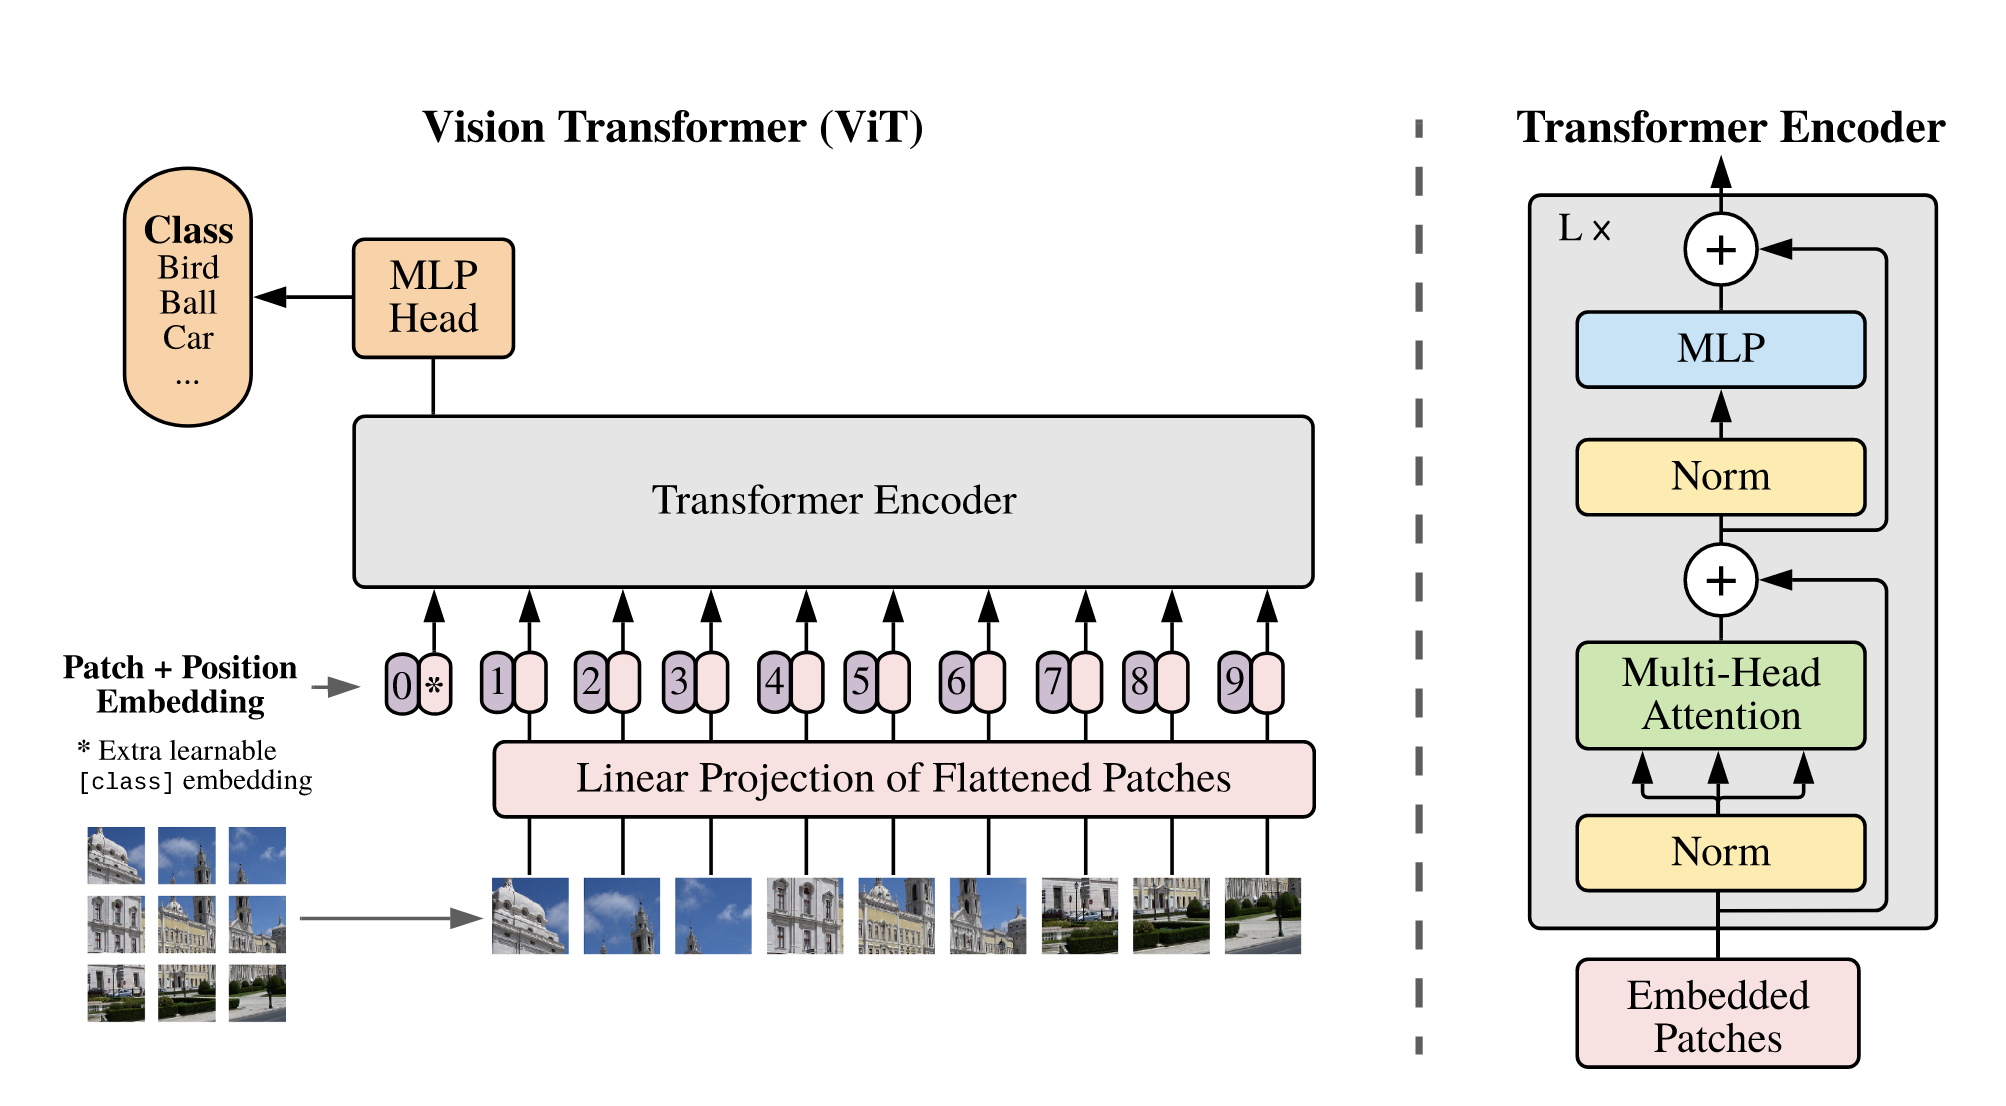
\includegraphics[width=\linewidth]{images/related/vit.png}
      \end{center}
      \caption{\textbf{The Vision Transformer (ViT):} the image is cropped without overlap and
            projected using a convolution whose stride equals the kernel size. The encoder is made of
            multiple transformer blocks. Finally, only the special learned token ``class token'' is used
            at the end, and fed to a linear classifier. Image from \cite{dosodosovitskiy2020vit}.}
      \label{fig:related_vit}
\end{figure}

More recently, the Transformer architecture \citep{vaswani2017transformer}, originally designed for
machine translation in \ac{NLP}, was applied to images. Using an encoder structure similar to BERT
\citep{devlin2018bert}, ViT \citep{dosovitskiy2020vit}, illustrated in \autoref{fig:related_vit},
considered patches of pixels as tokens. A special learned token, called ``class token'' is added to
the patch tokens. All the tokens are then processed through multiple transformer blocks. Each block
is made of LayerNorm \citep{ba2016layernorm}, a \ac{MHSA}, a \ac{MLP}, and residual connections.
Given a single head, the Self-Attention is:
%
\begin{equation}
      \begin{aligned}
            Q & =W_{q} \vx\,,                                                       \\
            K & =W_{k} \vx\,,                                                       \\
            V & =W_{v} \vx\,,                                                       \\
            A & =\operatorname{Softmax}\left(Q \cdot K^{T} / \sqrt{D / h}\right)\,, \\
            O & = W_{o} A V+b_{o}\,.
      \end{aligned}
      \label{sec:related_sa}
\end{equation}
%
$\vx$ are the $N$ patch tokens and the class token, of shape $(N, D)$, $D$ being the embedding
dimension. The patch tokens are linearly transformed thrice in a \textbf{Q}uery, \textbf{K}ey, and
\textbf{V}alue. An attention matrix of shape $(N, N)$ is computed from the query and the key. Its
$i^{\text{th}}$ row contains the similarity between the $i^{\text{th}}$ with all other tokens.
Finally, the multiplication between the attention matrix and the value matrix averages all tokens
according to their similarities. To extend the Self-Attention its multi-heads variation, we use
several Query/Key/Value transformations and do as many self-attentions in parallel.

\section{Continual Learning}
\label{sec:related_continual}

Usually, when training a \ac{CNN}, we assume the dataset is immutable and \textit{i.i.d.}: no new
image nor new classes will be learned. The knowledge acquired on one dataset A can be
\textit{transferred} to another dataset B with different classes using \textbf{transfer learning}
\citep{razavian2014transferlearning}. However, in that case, the new model, while being efficient on
the dataset B, cannot classify the classes of dataset A.

\textbf{Continual Learning} aims to learn a continually changing dataset without forgetting the
previous knowledge. The distribution of the dataset continually change: at each time-step, \ac{NC},
\ac{NI} from potentially new domains, or even \ac{NIC} are added to the training dataset
\cite{lomonaco2017core50}. We usually assume the test dataset evolves similarly. Continually
learning an ever-growing dataset is doable: a naive but efficient approach consist in training from
scratch a new model on the union of past and new data. However, for multiple reasons like privacy
concerns of medical data or limited storage capacity in embedded device, there is a restriction on
the amount of previous data that can be kept. In the extreme case, where a model only has access to
new data but now old data, training from scratch fails to model previous iterations' distribution.
Worse, even if the old model is kept and finetuned on the new data, it'll suffer from
\textbf{Catastrophic Forgetting} \citep{robins1995catastrophicforgetting}: new data is learned at
the expanse of old data. Multiple distribution shifts exist in Continual Learning
\citep{morenotorresa2012datasetshift,lesort2021driftanalysis}, and they have been called under various names in the
literature. I detail now the major ones, given $x$ an input sample and $y$ its label:

\begin{itemize}
      \item \textbf{Covariate shift}: when $p(x)$ changes, also known as domain incremental.
      \item \textbf{Prior shift}: when $p(y)$ changes; \ac{CIL} happens with this kind of shift.
      \item \textbf{Conceptual shift}: when $p(y | x)$ changes. Seldom covered in the literature, it
            can be found in \acf{CSS}.
\end{itemize}

In the chapter \autoref{chapter:regularization} and \autoref{chapter:dynamic}, I tackled only the
prior shift, while in \autoref{chapter:segmentation} I solved all three described shifts.


\paragraph{Class-Incremental Example} More concretely, a common benchmark in \ac{NC} setting,
commonly called \ac{CIL} is to learn the image classification CIFAR100 dataset
\citep{krizhevskycifar100} in multiple steps, each made of several new classes. \eg a model could
learn at first to classify among 10 classes, then add 10 more classes, \etc. until it has learned
all 100 classes. After each step, the model has to classify among all classes it has learned. The
\autoref{fig:related_forgetting} illustrate such continual training. The \textcolor{orange}{orange}
line displays the accuracy of a model that is re-trained from scratch at each step on all previous
classes data. This model, usually called Joint, is considered as a reasonable upper bound. The
\textcolor{blue}{blue} line on the other hand is a model that is finetuned on new classes but has no
access to previous classes. Evidently, the model's accuracy is much lower than its Joint
counterpart, because it forgets completely old classes by over-predicting new classes.

\paragraph{Single-Head \vs Multi-Heads} are the two main evaluation settings in Continual Learning
\citep{chaudhry2018riemannien_walk}. In the former setting, a model has to classify samples among
all seen classes, that could have been learned from any of the seen steps. The latter setting, on
the other hand, knows at test-time from which steps the samples come from. Thus, it only has to
classify among the limited number of classes brought by a step. This setting is closely related to
multi-tasks learning. During this thesis, I focused on the Single-Head setting because it's more
realistic as it's not always possible to know from which step a sample come from in a real-life
setting, and more challenging \citep{lesort2019regulshortcomings}.

\begin{figure}[tb]
      \begin{center}
            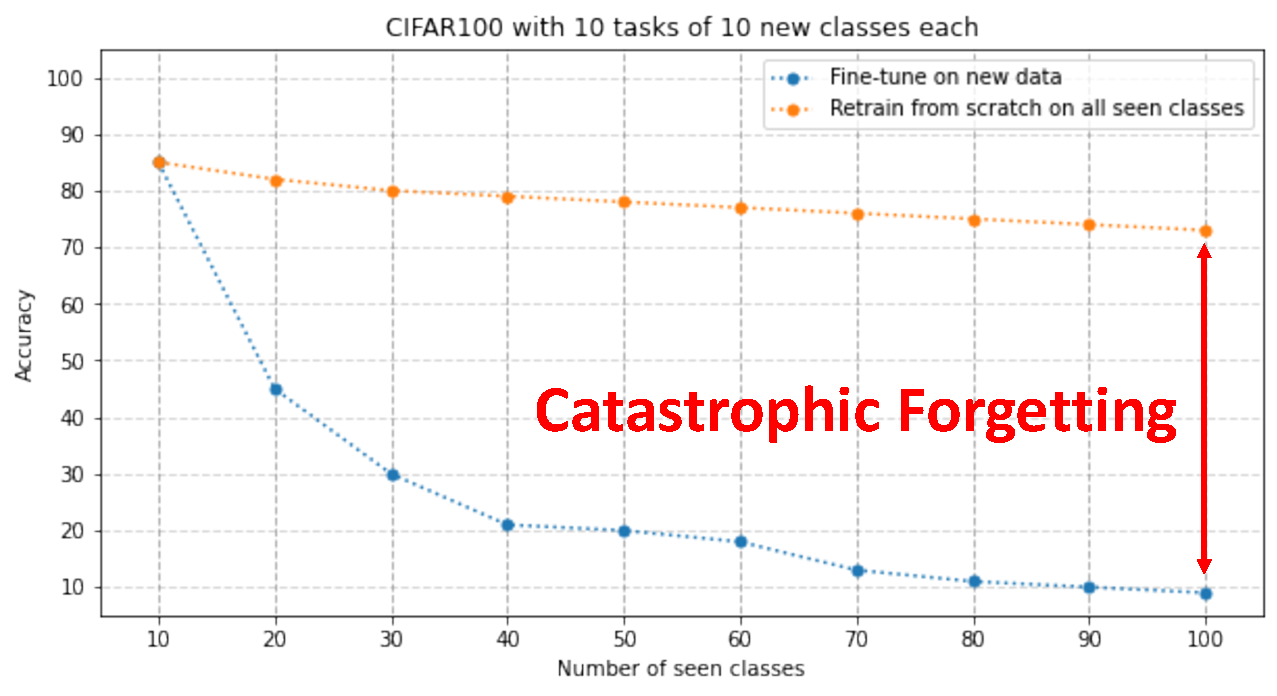
\includegraphics[width=0.8\linewidth]{images/related/catastrophic_forgetting.pdf}
      \end{center}
      \caption{\textbf{Training protocol for incremental learning}. At each training task we learn a
            new set of classes, and the model must retain knowledge about \textit{all} classes. The
            model is allowed a \textit{limited} memory of samples of old classes.}
      \label{fig:related_forgetting}
\end{figure}

\paragraph{Notations} I define in \autoref{tab:related_notation} the notations used thorough this thesis.

\begin{table}[t]
    \centering
    \begin{tabular}{@{}l|c@{}}
        \toprule
        Total number of tasks              & $T$                                      \\
        Current task                       & $t$                                      \\
        Current classes                    & $\mcC^t$                                 \\
        Previous classes                   & $\mcC^{1:t-1}$                           \\
        Future classes                     & $\mcC^{t+1:T}$                           \\
        Cardinality of a set of classes    & $\mcN^t=\operatorname{card}(\mcC^{t})-1$ \\
        Image and label maps at task $t$   & $\vx^t$ and $\y^t$                       \\
        Feature extractor at task $t$      & $f^t(\cdot)$                             \\
        Classifier at task $t$             & $g^t(\cdot)$                             \\
        Learnable parameters at task $t$   & $\Phi^t$                                 \\
        Predicted labels                   & $\hat{y}^t$                              \\
        Intermediary features at level $l$ & $f^t_l,\,l \in \{1, \dots, L\}$          \\
        \bottomrule
    \end{tabular}
    \caption{Notations used in this paper.}
    \label{tab:related_notation}
\end{table}


\subsection{Metrics for Continual Learning}
\label{sec:related_metrics}

\epigraph{If you cannot measure it, you cannot improve it.}{\textit{Lord Kelvin}}

Multiple metrics exist in Continual Learning: the most common are the \textbf{final accuracy} and
\textbf{average incremental accuracy}. The former measures the performance of the model on all tasks
at the last step. The latter measures the average of performance on all seen tasks after each new
task learned \citep{rebuffi2017icarl}. Practically, given $A_{i,t}$ the accuracy of the $i^{th}$
task after
learning the $t^{th}$ task, the final accuracy is (assuming balanced tasks):
%
\begin{equation}
      \text{Acc}_F = \frac{1}{T} \sum_{i=1}^T A_{i,T}\,,
      \label{eq:related_final_acc}
\end{equation}
%
and the average incremental accuracy:
%
\begin{equation}
      \text{Acc}_a = \frac{1}{T} \sum_{t=1}^T \frac{1}{t}  \sum_{i=1}^t A_{i,t}\,.
      \label{eq:related_avg_acc}
\end{equation}
%
Average incremental accuracy is somewhat more important than simply the final accuracy: a continual
model should be good after every step, as in a true continual setting there are no "final task".

Multiple other metrics exists \citep{diaz2018continualmetrics}, including the \textbf{backwardø and forward transfer} \citep{lopezpaz2017gem}
that measures the influence that learning a task has on the performance of respectively past and
future tasks. Another notable metric is the \textbf{forgetting} \citep{chaudhry2018riemannien_walk}
which records how much a model has lost performance-wise on a task compared to the first time it has
learned it. The interest of this metric is to be agnostic of the absolute performance of the model used.

Finally, metrics such as \textbf{speed} or used \textbf{capacity} are important: \cite{ramasesh2022scalecontinual}
recently showed that the larger a model was the lower was the forgetting.

\section{Methods to reduce forgetting}
\label{sec:related_methods}

\subsection{Rehearsal}
\label{sec:related_rehearsal}

Multiple approaches exist to reduce catastrophic forgetting. The most efficient method is
\textbf{rehearsal learning} where old samples will be seen alongside the new samples. The amount of
old samples stored is extremely limited otherwise it would defect the purpose of continual learning.
\autoref{fig:related_protocol} illustrates how rehearsal learning happens in Continual Learning.
During the first step, a model is trained on all available samples. Then, it stores a limited amount
of those in a \textit{memory}. During the second step, the model has access to new samples but also
all samples stored in the memory. In Class-Incremental, an equal amount of samples per class is
stored in memory. Nevertheless, there are two major approaches to determine this amount:
\cite{rebuffi2017icarl} proposed to fully use a memory of size $\mcM$ among all $\mcC$, while
\cite{hou2019ucir} instead kept fixed the amount of samples stored per class to $\nicefrac{\mcM}{|\mcC|}$.

\paragraph{Herding} is the action of choosing which samples per class to store in the rehearsal
memory. The most naive herding method is to sample randomly images. Despite its simplicity, it's
quite competitive with more complex method \citep{castro2018end_to_end_inc_learn}, echoing similar
results in \ac{AL} \citep{gal2017activelearning}. Other herding methods include fetching samples
close to the class mean in the feature space \citep{castro2018end_to_end_inc_learn} or close to an
incremental barycenter \citep{rebuffi2017icarl}.

\paragraph{Sampling} is an important but yet fewly investigated topic in Continual Learning. Most
models mix all memory samples with new samples without any under- or over-sampling.
\cite{castro2018end_to_end_inc_learn} propose to finetune for a few epochs, after training on a new
step, on a balanced set of old and new classes samples. \cite{chaudhry2019tinyepisodicmemories}
oversample tiny memory with as low as one sample per class, and show, in the context of Online
Learning (\autoref{sec:related_online_learning}), that continual models still don't overfit. In the
same context, \cite{aljundi2019maximallyinterfered} proposed to over-sample the memory examples with
highest losses. In an imbalanced situation for Continual Learning, over- and under-sampling can be
applied depending on the amount of samples per classes \citep{kim2020imbalancedcontinual}.

\paragraph{Efficient Storing} is important for rehearsal learning: a bigger rehearsal memory leads
invariably to less forgetting \citep{douillard2020podnet}. Thus, several works considered how more
samples could be stored given the same memory size: \cite{hayes2020remind} compress intermediate
features of memory samples with a lossless compression algorithm.
\cite{iscen2020incrementalfeatureadaptation} also store features but modify them through the
training to handle the inherent internal covariate shift. \cite{douillard2021objectrehearsal}, in
the context of segmentation, store only non-regular patches of zones of interest instead of storing
the whole, large, images.

\paragraph{Pseudo-rehearsal} doesn't need to store samples, but instead generates pseudo-samples for
rehearsal \citep{lesort2019generative}. The generation can be done with auto-encoders from
intermediate features \citep{kemker2018fearnet,ayub2021eec} or use \ac{GAN}
\citep{shin2017deep_generative_replay}. Those methods unfortunately have several drawbacks: they
struggle to scale to large images, the generator size may be superior to a classic rehearsal memory
size which would defeat the goal of using less storage, and finally the generator may itself suffer
from catastrophic forgetting. \cite{liu2020mnemonics} propose instead a method halfway between
rehearsal and pseudo-rehearsal: the authors sample randomly real images, and then during continual
training, slightly modify them via bi-level optimization to minimize forgetting.


\begin{figure}[tb]
      \begin{center}
            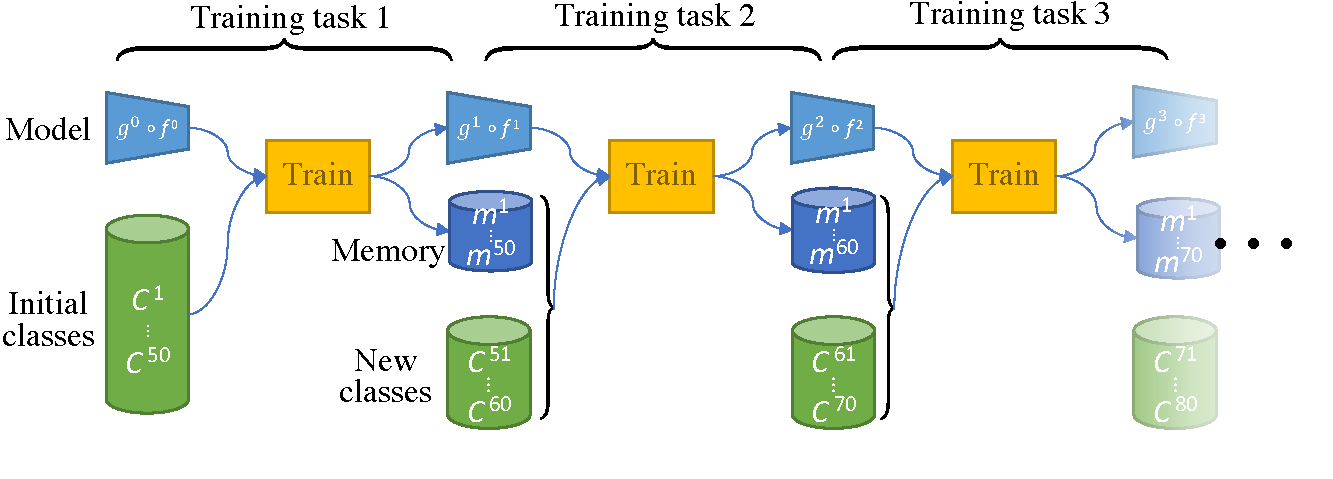
\includegraphics[width=1.0\linewidth]{images/podnet/protocol}
      \end{center}
      \caption{\textbf{Training protocol for incremental learning}. At each training task we learn a
            new set of classes, and the model must retain knowledge about \textit{all} classes. The
            model is allowed a \textit{limited} memory of samples of old classes.}
      \label{fig:related_protocol}
\end{figure}

\autoref{fig:related_protocol}


\subsection{Regularization-based Approaches}
\label{sec:related_regul}


\begin{figure}[tb]
      \begin{center}
            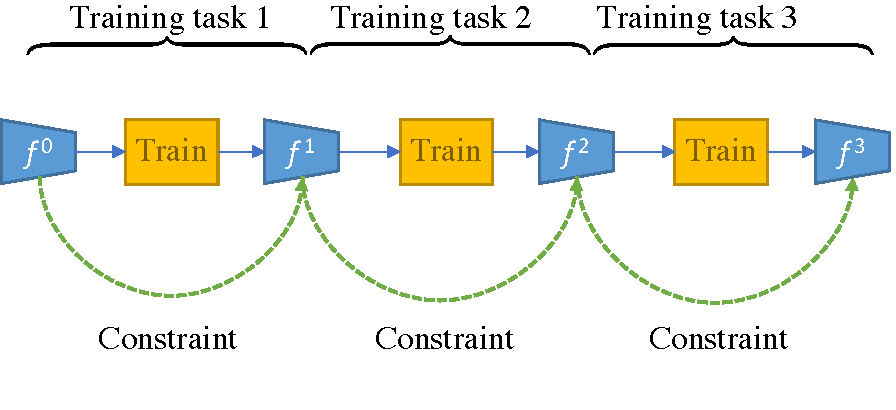
\includegraphics[width=1.0\linewidth]{images/related/continual_regularizations.pdf}
      \end{center}
      \caption{\textbf{Regularizations constraints} forcing the new model to be \textit{similar} to
            the old model to reduce catastrophic forgetting.}
      \label{fig:related_regul}
\end{figure}

A common and efficient way to reduce forgetting, is to minimize the difference in behavior between
the old and new models as illustrated in \autoref{fig:related_regul}. These constraints can be
expressed through various forms as described below.

\subsubsection{Weight-based}
\label{sec:related_regul_weight}


The most straightforward way to avoid completely forgetting, is that the old and new
models are identical. While the model would be \textit{rigid} (no forgetting), it is also not
\textit{plastic} at all, and thus cannot learn any new tasks. Thus, a line of research proposed to
constrain only a portion of the neurons:
%
\begin{equation}
      \mcL(\theta) = \mcL_\mcT(\theta) + \lambda \sum_i \Omega_i (\theta_i - \theta_i^*)^2\,,
      \label{eq:related_weight_constraint}
\end{equation}
%
where $\mcL_\mcT(\theta)$ is the loss of the current task (\eg the cross-entropy), $\theta_i$ and
$\theta_i^*$ respectively the $i^\text{th}$ neuron of the current and previous model, and $\Omega_i$
a neuron-wise importance factor. The intuition is that important neuron for $\mcT-1$ shouldn't
change, while the others can be adapted to fit the new task $\mcT$.

\cite{kirkpatrick2017ewc}, followed by
\cite{zenke2017synaptic_intelligence} and \cite{chaudhry2018riemannien_walk}
proposed to use the diagonal Fisher information matrix as importance factors.
\cite{aljundi2018MemoryAwareSynapses} instead used the sensitivity of the model when
small perturbations are added to the neurons to measure their importance.

However, it's worth remarking that weight-based constraints are usually limited to the multi-heads
setting where a task identifier is available at test time. \cite{lesort2019regulshortcomings} showed
that in the more realistic single-head setting, they barely reduce forgetting and were significantly
outperformed by rehearsal-based methods.

\subsubsection{Gradient-Based}
\label{sec:related_regul_gradient}

\begin{figure}[tb]
      \begin{center}
            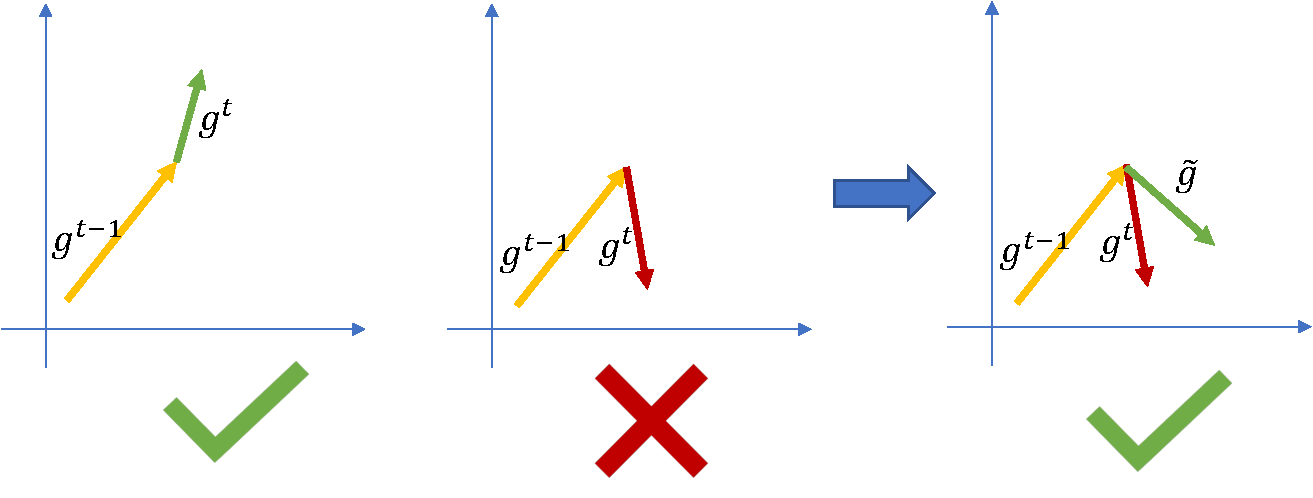
\includegraphics[width=1.0\linewidth]{images/related/gem.pdf}
      \end{center}
      \caption{\textbf{GEM's gradient constraint} forcing updates to be in the same direction as the
            gradient \wrt old samples.}
      \label{fig:related_gem}
\end{figure}

\cite{lopezpaz2017gem} proposed the GEM model which combines a constraint on the gradients and
rehearsal learning. The algorithm requires that the loss on a given stored sample must not increase
despite the model learning new classes. The authors, given a locality assumption, rewrite this
formulation as enforcing that the gradient of a new sample ($g$) to be in the same \textit{direction} as
the gradient of a stored old sample ($g_i$):
%
\begin{equation}
      \langle g,\, g_i\rangle \ge 0,\, \text{for all} i \in \mcM
\end{equation}
%
With $\mcM$ the rehearsal memory. If the constraint is violated, the new gradient $g$ is projected
to the closest in L2 norm gradient that satisfies the angle constraint by minimizing a quadratic
program. The constraint is illustrated in \autoref{fig:related_gem}. The drawback of this method is
the computational cost that can grow prohibitively when the memory is too large.
\cite{chaudhry2019AGEM} proposed Averaged-GEM to speed up GEM: the author don't constraint the
gradient of individual memory samples but only the average of all memory samples.
\cite{aljundi2019gradientselection} also improved GEM's speed by selecting only a subset of the
memory samples that maximize the feasible region.

Differently, but still constraining the gradients: \cite{farajtabar2020ogd}'s OGD forces the gradients of
task $t$ to be orthogonal to gradients of task $t-1$. They use the Gram-Schmidt procedure to
orthogonalize the new gradients, allowing updates for the new task that minimally interfere with the
performance of old tasks. \cite{saha2021gpm}'s GPM does likewise but using instead a k-rank
approximation of the SVD of the representation matrix.


\subsubsection{Output-based}
\label{sec:related_regul_output}

Finally, the majority of Continual model that are benchmarked on large datasets (\eg ImageNet
\citep{deng2009imagenet}, Pascal VOC \citep{everingham2015pascalvoc}) use a combination of rehearsal
learning (\autoref{sec:related_rehearsal}) and constraints on the model's outputs.

LwF \cite{li2018lwf} and iCaRL applied the \ac{KD} \cite{hinton2015knowledge_distillation} on the
model's probabilities. It usually consists in minimizing the \ac{KL} between the probabilities
of the old and new models:
%
\begin{equation}
      \mcL_\text{KD} = \operatorname{KL}(\operatorname{softmax}(\frac{\tilde{y}^{t-1}}{\tau}) \Vert \operatorname{softmax}(\frac{\tilde{y}^t}{\tau})\,,
\end{equation}
%
where $\tilde{y}^{t-1}$ and $\tilde{y}^{t}$ are respectively the logits of the old and new model,
and $\tau$ a \textit{temperature} to soften the probabilities in order to give more importance to
the \textit{dark knowledge} of \cite{hinton2015knowledge_distillation}. Note that in the context of
Class-Incremental, the new model predicts more classes than the old model, therefore the \ac{KL} is
only applied on the logits common to both the old and the new models. The \ac{KD} is sometimes also
defined as the binary cross-entropy between the sigmoid-activated logits.

Constraining the probabilities is now so ubiquitous that most models include it in their base
losses. On the other hand, a few models considered constraining intermediate outputs. MK2D
\citep{peng2019m2kd} uses the \ac{KD} from both the final classifier and an auxilliary classifier
similarly to the Inception network \citep{szegedy2015inception}. \cite{hou2019ucir} maximizes the
cosine similarity between the embeddings produced by the \ac{GAP}.
\cite{dhar2019learning_without_memorizing_gradcam} minimizes the L1 distance between the attention
maps produced by GradCam \citep{selvaraju2017gradcam}. Drawing inspiration from the model
compression litterature \cite{zagoruyko2016distillation_attention}, \cite{douillard2020podnet}
proposed to constraint instead the statistics of all intermediate features of the \ac{ConvNet}. This
constraint was later expanded to incorporate multiscale information \cite{douillard2020plop}.

\subsection{Structural Strategies}
\label{sec:related_structural}

\begin{figure}[tb]
      \begin{center}
            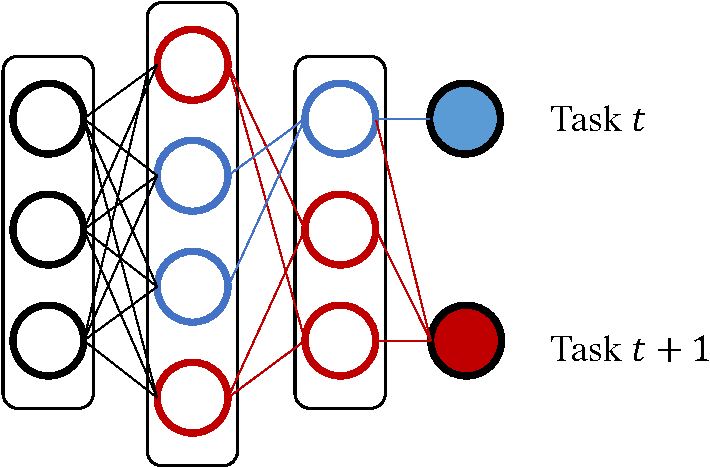
\includegraphics[width=0.6\linewidth]{images/related/subnetworks.pdf}
      \end{center}
      \caption{\textbf{Task-specific subnetworks} that can be uncovered with a sparsity loss or
            learned masking.}
      \label{fig:related_subnetwork}
\end{figure}

Multiple works have also proposed to adopt dynamic strategies where the configuration of the neural
network is different for each task to learn.

\paragraph{Subnetworks} The Lottery Ticket Hypothesis \citep{frankle2019lottery_ticket} states that
subnetworks, made of a fraction of the neurons and connections of a larger network, can reach
excellent performance. Several Continual Learning models have exploited that property by using a
subnetwork per task. Those subnetworks can be uncovered via genetic algorithms
\citep{fernando2017path_net}, via induced L1 sparsity \citep{golkar2019neural_pruning}, or even
learned masked \cite{serra2018hat,hung2019cpg}. Usually, these methods require a task identifier at
test-time in order to select the right subnetwork (see \textit{multi-heads} in
\autoref{sec:related_continual}). Later, \cite{wortsman2020supermasks} proposed to infer the task
identifier by selecting the subnetwork with the lowest entropy. This subnetwork-based approach is
illustrated in \autoref{fig:related_subnetwork}.

\paragraph{Expandable Networks} A neural network can also be expanded thorough its continual
training to accommodate the growing amount of tasks to solve. First, \cite{rusu2016progressive}
proposed to have one network per task, where the $i^{\text{th}}$ network would depend both on the
input and all previous networks' intermediate features. Unfortunately, the memory consumption is
quickly prohibitive with many tasks. Following works have proposed to only add blocks of parameters,
and only when deemed necessary
\citep{hung2019cpg,veniat2021mntdp,ostapenko2021localmodulecomposition}.

\paragraph{Task Conditioning} Rather than adding many new parameters, it's also possible to only add
a few parameters that will adapt the existing network \citep{rebuffi2017visualadapters}:
\cite{wen2020batchensemble} and \cite{sun2019metatransfer} proposed to share most of the weights
across tasks, but have task-specific weights that directly modify the shared weights.

\paragraph{Mixture-of-Experts} Mixture of experts \citep{masoudnia2014mixture} have also been
proposed, where multiple experts combine their decision. \cite{aljundi2017experts} learn a gating
system to use the right task-specific expert. \cite{yan2021der} and \cite{li2021preserve} proposed
to have a \ac{ConvNet} per task, and to concatenate their output embeddings to be fed to a single
classifier. To avoid parameters explosion, they aggressively prune each \ac{ConvNet}.

\paragraph{Classifier Correction} Forgetting happen in both the feature extractor and the
classifier. Previously described rehearsal and regularization methods try to reduce it in both
places. On the other hand, multiple works focused solely on the classifier. They remarked that in
\acf{CIL}, the classifier is miscalibrated \citep{guo2017miscalibration} where the model
over-predicts new classes to the detriment of old classes. \cite{belouadah2019il2m} compensate the
bias towards new classes by rectifying predictions of past classes using their recorded accuracies
and confidences. \cite{wu2019bias_correction} learn a linear model on validation data to recalibrate
the logits of the new classes. \cite{zhao2020weightalignement} normalizes the norm of the classifier
weights associated to new classes so that their average norm becomes the same as that for old
classes. \cite{hou2019ucir}, aims for a similar result, by replacing the dot product in the
classifier by a cosine similarity, resulting in classifier weights of unit norm for all.

